\documentclass[draft,grl]{agutexSI2019}


%IMPORTANT NOTE ON FIGURES AND TABLES
% Placeholders for figures and tables appear after the \end{article} command, after references.
% DO NOT USE \psfrag or \subfigure commands.
%
 \usepackage{graphicx}
 \usepackage{amsmath}
 \usepackage{amssymb}
 \usepackage{bm}
 
 \newcommand{\norm}[1]{\left\lVert#1\right\rVert}
 
\renewcommand{\thetable}{S\arabic{table}}
\renewcommand{\thefigure}{S\arabic{figure}}
\renewcommand{\thesection}{S\arabic{section}}
%
%  Uncomment the following command to allow illustrations to print
%   when using Draft:
 \setkeys{Gin}{draft=false}
%
% You may need to use one of these options for graphicx depending on the driver program you are using. 
%
% [xdvi], [dvipdf], [dvipsone], [dviwindo], [emtex], [dviwin],
% [pctexps],  [pctexwin],  [pctexhp],  [pctex32], [truetex], [tcidvi],
% [oztex], [textures]
%
%
%% ------------------------------------------------------------------------ %%
%
%  ENTER PREAMBLE
%
%% ------------------------------------------------------------------------ %%

% Author names in capital letters:
\authorrunninghead{Staniewicz ET AL.}

% Shorter version of title entered in capital letters:
\titlerunninghead{InSAR surface deformation in the Permian Basin}

%Corresponding author mailing address and e-mail address:
\authoraddr{Corresponding author: Scott Staniewicz, 
Department of of Aerospace Engineering and Engineering Mechanics, The University of Texas at Austin, 
Austin, TX 78712, USA.
(scott.stanie@utexas.edu)}

\begin{document}

%% ------------------------------------------------------------------------ %%
%
%  TITLE
%
%% ------------------------------------------------------------------------ %%

%\includegraphics{agu_pubart-white_reduced.eps}


\title{Supporting Information for ``InSAR reveals complex surface deformation patterns over an 80,000 square kilometer oil-producing region in the Permian Basin''}

%% ------------------------------------------------------------------------ %%
%
%  AUTHORS AND AFFILIATIONS
%
%% ------------------------------------------------------------------------ %%

\authors{
Scott Staniewicz\affil{1},
Jingyi Chen\affil{1},
Hunjoo Lee\affil{2},
Jon Olson\affil{2},
Alexandros Savvaidis\affil{3},
Robert Reedy\affil{3},
Caroline Breton\affil{3},
Ellen Rathje\affil{4},
Peter Hennings\affil{3}
}

\affiliation{1}{Department of Aerospace Engineering and Engineering Mechanics, The University of Texas at Austin, Austin, TX 78712}
\affiliation{2}{Hildebrand Department of Petroleum and Geosystems Engineering, The University of Texas at Austin, Austin, TX 78712}
\affiliation{3}{Bureau of Economic Geology, The University of Texas at Austin, Austin, TX 78758}
\affiliation{4}{Department of Civil, Architectural, and Environmental Engineering, The University of Texas at Austin, Austin, TX, 78712}

\begin{article}


\noindent\textbf{Contents of this file}
%%%Remove or add items as needed%%%
\begin{enumerate}
\item Section S1 to S7
\item Tables S1 to S4
\item Figures S1 to S12
%if Tables are larger than 1 page, upload as separate excel file
\end{enumerate}

\clearpage

\section{Shale development and induced seismicity in the Permian Basin}
\label{sec:background}
The success of shale development technologies \cite{Waters2006use} has opened up vast shale resources for economically viable oil and gas production. Based on a recent assessment by the U.S. Geological Survey (USGS), the Wolfcamp shale in Texas' Permian Basin is the largest continuous oil field that has ever been discovered in the United States \cite{GaswirthAssessment2016}. As of 2017, there were over 130,000 active production wells, 23,041 active enhanced oil production (EOR) wells, and 3794 active saltwater disposal (SWD) wells in the Permian Basin (Figure \ref{fig:Permian} (a)). It has been recognized that injection or withdrawal of fluids from the subsurface can induce earthquakes along existing faults \cite{Ellsworth2013, simpson1988two}. While petroleum production and wastewater injection volumes have been rising throughout the basin, the recently-cataloged earthquakes are spatially clustered (Figure \ref{fig:Permian} (b)-(f)). One significant cluster is near Pecos, TX, where increased seismic activity began in 2009 \cite{Frohlich2019}. Subsequent activity has increased considerably, with \citeA{skoumal2020induced} identifying more than 500 earthquakes 2017 and over 1000 earthquakes in 2018.


\section{InSAR line-of-sight decomposition}
\label{sec:los}
An interferogram measures surface deformation between the two SAR acquisition times along the radar line-of-sight (LOS) direction \cite{Hanssen2001}. The LOS deformation, $u_{LOS}$, can be written as: 
\begin{align}
u_{LOS}= \alpha_{e} u_{e} + \alpha_{n} u_{n} + \alpha_{u} u_{u}
\end{align}
where $u_{e}$, $u_{n}$ and $u_{u}$ are the east, north and up displacements, respectively. The radar look vector $\alpha = [\alpha_e, \alpha_n, \alpha_u]$ can be calculated from the known imaging geometry at every pixel location. This varies significantly across the basin due to the $ \sim$250 km wide Sentinel swath (Figure \ref{fig:los-map}). 

In regions where InSAR data are available from two LOS directions, we can decompose the ground motion into its eastward and vertical components.
To perform the decomposition, we first write $u_{asc}$ and $u_{desc}$ in terms of $u_e$, $u_n$ and $u_u$:
\begin{align}
    u_{asc} &= \alpha_{a,e} u_{e} + \alpha_{a,n} u_{n} + \alpha_{a,u} u_{u}\\
    u_{desc} &= \alpha_{d,e} u_{e} + \alpha_{d,n} u_{n} + \alpha_{d,u} u_{u}
\end{align}
We can express $u_e$ and $u_u$ as:
\begin{align}
    u_{e} &\approx  \frac{1}{\beta}  \left[\alpha_{d,u}  u_{asc} - \alpha_{a,u} u_{desc} \right] \\
    u_{u} &\approx  \frac{1}{\beta}  \left[\alpha_{a,e} u_{desc} - \alpha_{d,e}  u_{asc}  \right] 
\end{align}
where  $ \beta = {\alpha_{a,e} \alpha_{d,u}- \alpha_{d,e} \alpha_{a,u}} $.

Because Sentinel-1 satellites are operating in a near-polar orbit, the north look coefficients $\alpha_{a,n}$ and $\alpha_{d,n}$ are both relatively small. Ignoring 1 cm northward motion in $u_n$ only leads to $\sim$ 0.1-0.2 mm error in $u_e$ and $\sim$ 1 mm error in $u_u$ at most locations. \citeA{Kim2018} detected several localized deformation features within the Delaware Basin related to wastewater injection, CO2 injection, and hydrocarbon production using Sentinel-1 InSAR data.  Our LOS decomposition results are consistent with their study at these locations. For example, in a 12 km x 12 km region centered on a wastewater injection well, we observed $\sim$ 5.5 cm of uplift and $\sim$1.2 cm of east-west motion between November 2014 and April 2017 (Figure \ref{fig:injection-kim-lu}). 

\clearpage
\section{The impact of the stratified component of tropospheric noise}
\label{sec:noise-quant}
The Generic Atmospheric Correction Online Service (GACOS) is an iterative tropospheric decomposition model that integrates global weather models and available GPS zenith delay measurements for estimating tropospheric noise in InSAR data \cite{yu2018interferometric}. Due to the limited spatial and temporal resolution of weather models and GPS data, GACOS is more effective in removing the stratified tropospheric noise \cite{Doin2009} than the random turbulent tropospheric noise \cite{Emardson2003}. We found that GACOS does not produce any substantial corrections on Sentinel-1 West Texas interferograms (e.g. Figure \ref{fig:GACOS} (a)-(c)). This is because the oil-producing region of the Permian Basin is relatively flat, and we observed little correlation between InSAR LOS measurements and the Digital Elevation Model (DEM) data (e.g. Figure \ref{fig:GACOS} (d)). We thus concluded that the stratified tropospheric noise was minimal in our study region.


\section{InSAR LOS velocity estimation errors using the stacking method}
\label{sec:error-quant}
We used independently processed GPS east, north, and up GPS time series as ground truth to quantify errors in the InSAR stacking solutions before and after the outlier removal. There are 13 permanent GPS stations in the ascending SAR footprint. At each GPS location, we projected the GPS time series to the radar line-of-sight (LOS), and we computed the GPS-inferred average LOS velocity through a linear regression. Table \ref{tab:gps-error-78} shows the root mean square (RMS) and the worst-case absolute differences between InSAR and GPS inferred average LOS velocities over the three study periods. Similarly, there are 5 permanent GPS stations in the descending SAR footprint, and Table \ref{tab:gps-error-85} shows the uncertainty in the descending stacking solutions using these 5 GPS stations as control. Both Table \ref{tab:gps-error-78} and Table \ref{tab:gps-error-85} show that our outlier removal algorithm reduced the uncertainty in InSAR stacking solutions by a factor of $\sim$2, down to 1-2 mm/year across the basin. For a given period of interest $T_j$, the LOS velocity error $ E_{vel,j} $ propagates into the cumulative deformation error $ E_{c, j} $ as $ E_{c,j} = E_{vel,j} \cdot T_j $. 


\section{A comparison between stacking and InSAR time series methods}
\label{sec:method-compare}
If data error treatments and deformation model assumptions are valid, we can derive meaningful and comparable deformation solutions using different InSAR time series analysis methods. To investigate how InSAR measurement noise influences the LOS deformation solutions, we compared the results derived from (1) the stacking method, (2) a Small BAseline Subset (SBAS) linear deformation (constant velocity) model with $L_1$ and $L_2$-norm penalty functions, and (3) unregularized and regularized SBAS deformation time series. 

For the remainder of this section, we assume there are $M$ small-baseline interferograms that were generated from $N$ SAR scenes acquired over a period of interest. The stacking method we employed in this study \cite{Sandwell1998} solves for the average velocity over the study period. Similarly, the SBAS linear deformation model solves for the average velocity $ v_{avg} $ over this period at each pixel of interest as \cite{SBAS2002}:
\begin{equation}
\arg \min_{v_{avg}} \norm{ \bm{BP} v_{avg} - \bm{d}   }_p
   \label{eq:sbas-linear}
\end{equation}
where $ \bm{B }$ is the $ M \times (N-1) $ SBAS matrix, $ \bm{P}$ is an $ (N-1) \times 1 $ vector of ones, $ \bm{d} $ is the $ M \times 1 $ vector of LOS measurements (in cm) at this pixel, and $ p \in \{1, 2\} $ is the norm used to penalize the data misfit. The $L_2$ linear deformation solution is comparable to the stacking solution (with an assumption of a constant velocity), and the $L_1$ solution is typically less sensitive to measurement outliers than the $L_2$ solution.

The LOS surface velocities between adjacent SAR acquisitions $ \bm{v} = \left[v_1 , \ldots , v_{N-1} \right]^T $ can be solved as:
\begin{equation}
\arg \min_{\bm{v} } \norm{ \bm{Bv} - \bm{d}   }^2_2 + \alpha \norm{ \bm{Dv} }^2_2  \label{eq:sbas}
\end{equation}
where $ \bm{D} $ is a $ (N-2) \times (N-1) $ matrix, with $1$ on the main diagonal and $-1$ on the superdiagonal, which approximates the first-order differentiation operator. The first term penalizes the data misfit, the second term is a temporal smoothness constraint, and $ \alpha \in \Bbb{R} $ is the weight between the two terms. When $ \alpha = 0 $, the solution is the unregularized SBAS deformation time series. An additional integration of $\mathbf{v}$ over time yields the LOS deformation time series.

Little surface deformation occurred between Nov. 2014 and Jan. 2019 at the 13 GPS permanent GPS stations. At each GPS location, we projected the GPS time series to the radar line-of-sight (LOS), and we used the GPS-inferred average LOS velocity (0-3 mm/year) as ground truth. Table \ref{tab:compare-errors} shows the root mean square (RMS) and the worst-case absolute differences between InSAR and GPS inferred average LOS velocities between Nov. 2014 and Jan. 2018 as derived from the four InSAR time series methods. We found that InSAR tropospheric noise has a strong influence on all the surface deformation solutions before removing the measurement outliers. As an example, Figure \ref{fig:compare} (a) shows the ascending LOS solutions between Nov. 2014 and Jan. 2018 at the GPS station TXSO before removing InSAR measurement outliers. The random tropospheric noise creates up to $\sim$6 cm of error in the unregularized SBAS surface deformation time series. This error can be reduced by increasing $ \alpha$ in Equation \eqref{eq:sbas}. As $\alpha$ increases, the LOS deformation time series converge to the $L_2$ linear deformation (constant velocity) solution. However, there are visible cm-level tropospheric artifacts in the cumulative deformation solutions by using either $L_1$ or $L_2$ linear deformation models (e.g. Figure 2 (d) in the main text). 

After removing InSAR outlier measurements associated with extreme local weather events as described in Section 2.3 (main text), all SBAS time series methods produce more accurate and consistent deformation trends (Figure \ref{fig:compare} (b)). The unregularized SBAS time series still contain up to $\sim$3 cm of tropospheric noise, which leads to long-wavelength artifacts in the basin-wide deformation maps. The $ L_1 $ and $ L_2 $ linear deformation solutions show close agreement ($<$ 2 mm difference) at all GPS stations. Since both methods suggest a deformation trend consistent with the stacking approach, we chose the simple stacking method as the final processing strategy for estimating cumulative surface deformation in the Permian Basin.


\section{ Dislocation (Fault Slip) Model}
\citeA{Okada1992} derived the analytical surface displacement field due to a finite rectangular fault slip in an elastic half-space. The Okada solutions provide three cases of displacement on a fault: strike-slip, dip-slip, tensile opening. In this study, we focused on the dip-slip case, because the Pecos area is in a normal faulting regime \cite{LundSnee2018}.  The assumption of predominant dip-slip along normal faults is also supported by fault plane solutions (TexNet Earthquake Catalog). 

Considering the case of dip slip on a finite rectangular fault (Figure \ref{fig:model-fault-geom}), the vertical surface displacement $u_z(x, y, 0)$ can be expressed as:
\begin{equation}
    u_{z}(x,y,0)=\frac{U_{2}}{2\pi }[u_{2}^{B}\sin \delta + u_{3}^{B}\cos \delta]
\label{eq:okada}
\end{equation}
where $U_2$ is the magnitude of dip slip. The rest of terms on the right are determined by fault geometry parameters: the fault dip angle ($\delta$), the depth to the top of the fault ($Z$), the fault width along the dip direction ($W$), and the fault length along the strike direction ($L$). 

We located four faults based on InSAR observations, and assumed a uniform slip on each fault. We estimated the best-fit fault parameters for each fault independently by minimizing the objective function \cite{Du1992}:
\begin{equation}
\arg \min_{U_{2,i}} \left \| \mathbf{G_i}U_{2,i}-\mathbf{d_i} \right \|^2_{2}  
\label{eq:model-obj-1}
\end{equation}	  	
where $\mathbf{G_i}$ is the discrete Green’s function that maps a dip slip, $U_{2,i}$, on the $i^{th}$ rectangular fault to the observed vertical deformation at specific surface locations.  $\mathbf{G_i}$ is a function of fault geometry parameters as shown in Equation \eqref{eq:okada}. $\mathbf{d_i}$ is a vector of vertical deformation observations associated with the $i^{th}$ fault from InSAR data.

Through a grid-search, we solved for the fault dip angle, the depth to the top of the fault, the width along the dip direction, and the magnitude of dip slip on each fault to minimize the sum of squared residuals normalized by the data error of 1 cm (Normalized Sum of Squared Residuals; NSSR). The fault length in the strike direction is set to be sufficiently long to satisfy the plane strain condition. As an example, Figure \ref{fig:fault-supplement-nssr} shows how the data misfit varies with fault parameters for fault \#3. The maximum R-squared ($R^2$) values for the best-fit fault parameters are in the range of 0.95 and generally agree with the fault parameters that satisfy the minimum NSSR. 

The best-fit fault parameters of the four faults are listed in Table \ref{tab:geo-mech-fault}, which produce 3D surface deformation patterns as shown in Figure \ref{fig:fault-model-xyz}. To illustrate how surface deformation observations are related to the model parameters, Figure \ref{fig:fault-supplement2} shows the estimated surface subsidence associated with the fault \#3 long the B-B' transect with various fault properties. The ratio of the uplift volume to the subsidence volume is a function of the seismic potency and the fault dip angle \cite{Segall2019integrated}. Based on the results in Figure \ref{fig:fault-supplement2} (a), the fault dip angle dominantly controls the uplift volume relative to the subsidence volume. The slope from the uplift on the footwall to the subsidence on the hanging wall becomes steeper as the fault becomes shallower (Figure \ref{fig:fault-supplement2} (b)). The fault width, as measured along the the dip direction, mostly contributes to the width of the subsidence bowl (Figure \ref{fig:fault-supplement2} (c)).  The dip-slip magnitude only has impact on the amplitude of the curve without any influence on the shape of the surface deformation (Figure \ref{fig:fault-supplement2} (d)).



\section{ Cylindrical Reservoir Compaction/Subsidence Model}
\label{sec:model-compact}
\citeA{Geertsma1973} derived the surface displacement field due to a uniform pressure drop of a cylindrical reservoir at a depth $D$ (Figure \ref{fig:model-reservoir-geom}). Under the assumption that the reservoir radius $R$ is larger than the reservoir height $H$, the cylindrical reservoir deforms primarily in the vertical direction. The magnitude of the reservoir compaction $\Delta H$ due to a pressure drop $\Delta P$ can be written as:
\begin{equation}
    \Delta H = H c_m \Delta P
\label{eq:rcompact}
\end{equation}
Here the  uniaxial compaction coefficient $c_m$ can be expressed as
\begin{align}
    c_{m} &= \alpha_{p}\frac{1+\nu}{1-\nu}\frac{c_{b}}{3} 
\end{align}
where $\alpha_p$ is Biot's coefficient, $c_b$ is the bulk compressibility, and $\nu$ is the Poisson's ratio. Surface vertical deformation $u_z$ due to the reservoir compaction $\Delta H$ can be expressed as:
\begin{align}
    u_{z}(r,0) &= 2(1-\nu)\Delta HA(\rho,\eta) 
    \label{eq:reservoirDef}
\end{align}
where $ A(\rho,\eta) = R\int_{0}^{\infty}e^{-D\alpha}J_{1}(\alpha R)J_{0}(\alpha r) \, d\alpha$, $\rho = r/R$, and $\eta =  D/R$. The maximum surface deformation at $r = 0$ can be written as:
\begin{equation}
    {u_{z}}^{max} = 2(1-\nu)\Delta H(1-\frac{\eta}{\sqrt{1+\eta^{2}}})
\end{equation}

The best-fit compaction in the cylindrical reservoirs were determined by minimizing the objective function \cite{Du2001}:
\begin{equation}
\arg \min_{\mathbf{\Delta H}} =\left \| \mathbf{G_R}\mathbf{\Delta H}-\mathbf{d_r} \right \|^2+\beta ^2\left \| \mathbf{H_L}\mathbf{\Delta H}-\mathbf{d_0} \right \|^2  \label{eq:model-obj-2}
\end{equation}
where $ \mathbf{G_R} $ is the discrete Green’s function that maps the compaction of cylindrical reservoirs $\mathbf{\Delta H}$ in the subsurface to the observed vertical deformation at specific surface locations. $\mathbf{G_R}$ is a function of reservoir geometry parameters as shown in Equation \eqref{eq:reservoirDef}. $\mathbf{d_r}$ is a vector of vertical deformation observations associated with the reservoir compaction. In this study, $\mathbf{d_r}$ is the difference between the InSAR-observed total vertical deformation and modeled vertical fault slip deformation, $ \beta^2 $ is the penalty factor that weights the smoothness constraint, and $ \mathbf{H_L} $ is the finite difference approximation of the Laplacian operator. The reservoir compaction is constrained to be negative, and $\mathbf{d_0} $ is set to be zero. 

Based on the production well data near Pecos, we discretized two layers of reservoirs in the subsurface: Delaware Mountain Group (DMG) at depth 1.52 km and Wolfcamp at depth 3.05 km (Figure \ref{fig:model-reservoir-wells}). The shallow groundwater level reservoirs were not included in the reservoir model, because the water levels in the groundwater aquifers in the Pecos area were stable over the time period of interest \cite{deng2020surface}. The producing wells in the DMG were predominantly located to the east of Pecos, and we set 25 cylindrical reservoirs with the radius of 0.83 km. In the Wolfcamp formation, the wells were producing over the entire region. We discretized the layer covering the entire area with 100 cylindrical reservoirs with the radius of 0.83 km.  

We utilized the pattern search optimization tool in MATLAB to minimize the objective function (Equation \eqref{eq:model-obj-2}). As the penalty factor $\beta^2$ decreases, the NSSR decreases, $ R^2 $ increases, and the modeled surface deformation better matches the InSAR data (Figure \ref{fig:model-reservoir-nssr}). Once the penalty factor ($ \beta^2 $) is smaller than 0.01, the NSSR and $ R^2 $ no longer change substantially. The best-fit reservoir compaction results ($ \beta^2 $ equals 0.01) for the two producing layers are shown in Figure \ref{fig:model-reservoir-wells}. While DMG reservoirs show some compaction (0 - 8 cm), the dominant compaction is in the Wolfcamp layer (0 - 27 cm). The production volume in DMG is as significant as in Wolfcamp. However, the dominant injection volume into DMG could maintain the reservoir pressure and minimize reservoir compaction. For certain regions in the Wolfcamp layer, the reservoir compaction appears to be discontinuous given the low $ \beta^2 $ value. We note that it is reasonable to observe localized compaction for tight shale formations, because the low formation permeability can cause heterogeneous pressure distribution during the depletion.

If appropriate mechanical properties of the formation are available, the distribution of reservoir pressure change and depleted zone can be evaluated by the reservoir compaction magnitudes based on Equation \eqref{eq:rcompact}. For example, if we assume Young’s modulus of 25 GPa, Poisson’s ratio of 0.25, and Biot’s coefficient of 0.67 based on published rock properties \cite{Shukla2013, Xu2015analysis}, the localized maximum pressure drop is approximately 21 MPa. This is within a reasonable range given operational history in the area.

% % % Tables % % %
\begin{table}
\caption{InSAR ascending LOS velocity estimation errors (in mm/year) using the stacking method}
\centering
\begin{tabular}{|c|c|c|}
\hline 
      & Before the outlier removal & After the outlier removal \\
      & (RMS / Worst) & (RMS / Worst) \\
      \hline
Nov. 2014 - Jan. 2017 & 3.8 / 9.5         & 1.9 / 5.9       \\\hline
Nov. 2014 - Jan. 2018 & 3.3 / 7.1         & 1.3 / 2.5       \\\hline
Nov. 2014 - Jan. 2019 & 2.0 / 6.1         & 1.1 / 2.5       \\\hline                
\end{tabular}
\label{tab:gps-error-78}
\end{table}

\begin{table}
\caption{InSAR descending LOS velocity estimation errors (in mm/year) using the stacking method}
\begin{tabular}{|c|c|c|}
\hline 
      & Before the outlier removal & After the outlier removal \\
      & (RMS / Worst) & (RMS / Worst) \\
      \hline 
Nov. 2014 - Jan. 2017 & 7.8 / 13.8                            & 2.9 / 5.0                          \\\hline
Nov. 2014 - Jan. 2018 & 3.7 / 7.5                             & 2.7 / 5.6                          \\\hline
Nov. 2014 - Jan. 2019 & 1.6 / 2.8                             & 0.8 / 1.6  \\\hline     
\end{tabular}
\label{tab:gps-error-85}
\end{table}

\begin{table}
\caption{Errors (in mm) in four SBAS ascending LOS deformation (Nov. 2014 - Jan. 2018) solutions}
\centering
\begin{tabular}{|c|c|c|}
\hline 
      & Before the outlier removal & After the outlier removal \\
      & (RMS / Worst) & (RMS / Worst) \\
      \hline
Unregularized &  22 / 99     &  14 / 43         \\\hline
Regularized   &    14 / 63   &   10  / 27       \\\hline
L1 linear deformation          &   7 / 11      & 4 / 8      \\\hline
L2 linear deformation          &   10 / 22        & 4 / 8      \\\hline
\end{tabular}
\label{tab:compare-errors}
\end{table}

\begin{table}
\centering
\caption{Best-fit fault parameters as derived from the dislocation model}
\begin{tabular}{c|cccc}
                    & Fault \#1      & Fault \#2      & Fault \#3      & Fault \#4      \\
\hline
1-Longitude ($^{\circ}$) & -103.563 & -103.589 & -103.585 & -103.529 \\
1-Latitude ($^{\circ}$)  & 31.367   & 31.413   & 31.463   & 31.470   \\
2-Longitude ($^{\circ}$) & -103.503 & -103.505 & -103.440 & -103.468 \\
2-Latitude ($^{\circ}$)  & 31.337   & 31.355    & 31.374   & 31.432   \\
Dip Angle ($^{\circ}$)   & 60       & 60       & 50       & 57.5       \\
Depth (km)               & 0.91     & 0.91     & 1.07     & 1.52     \\
Width (km)              & 0.61     & 0.30     & 1.07     & 0.61     \\
Slip (cm)                & 9.1     & 15.2     & 9.1     & 15.2    \\
\end{tabular}
\label{tab:geo-mech-fault}
\end{table}

% % % Figures % % %
\begin{figure*}[hbt!]
\centering
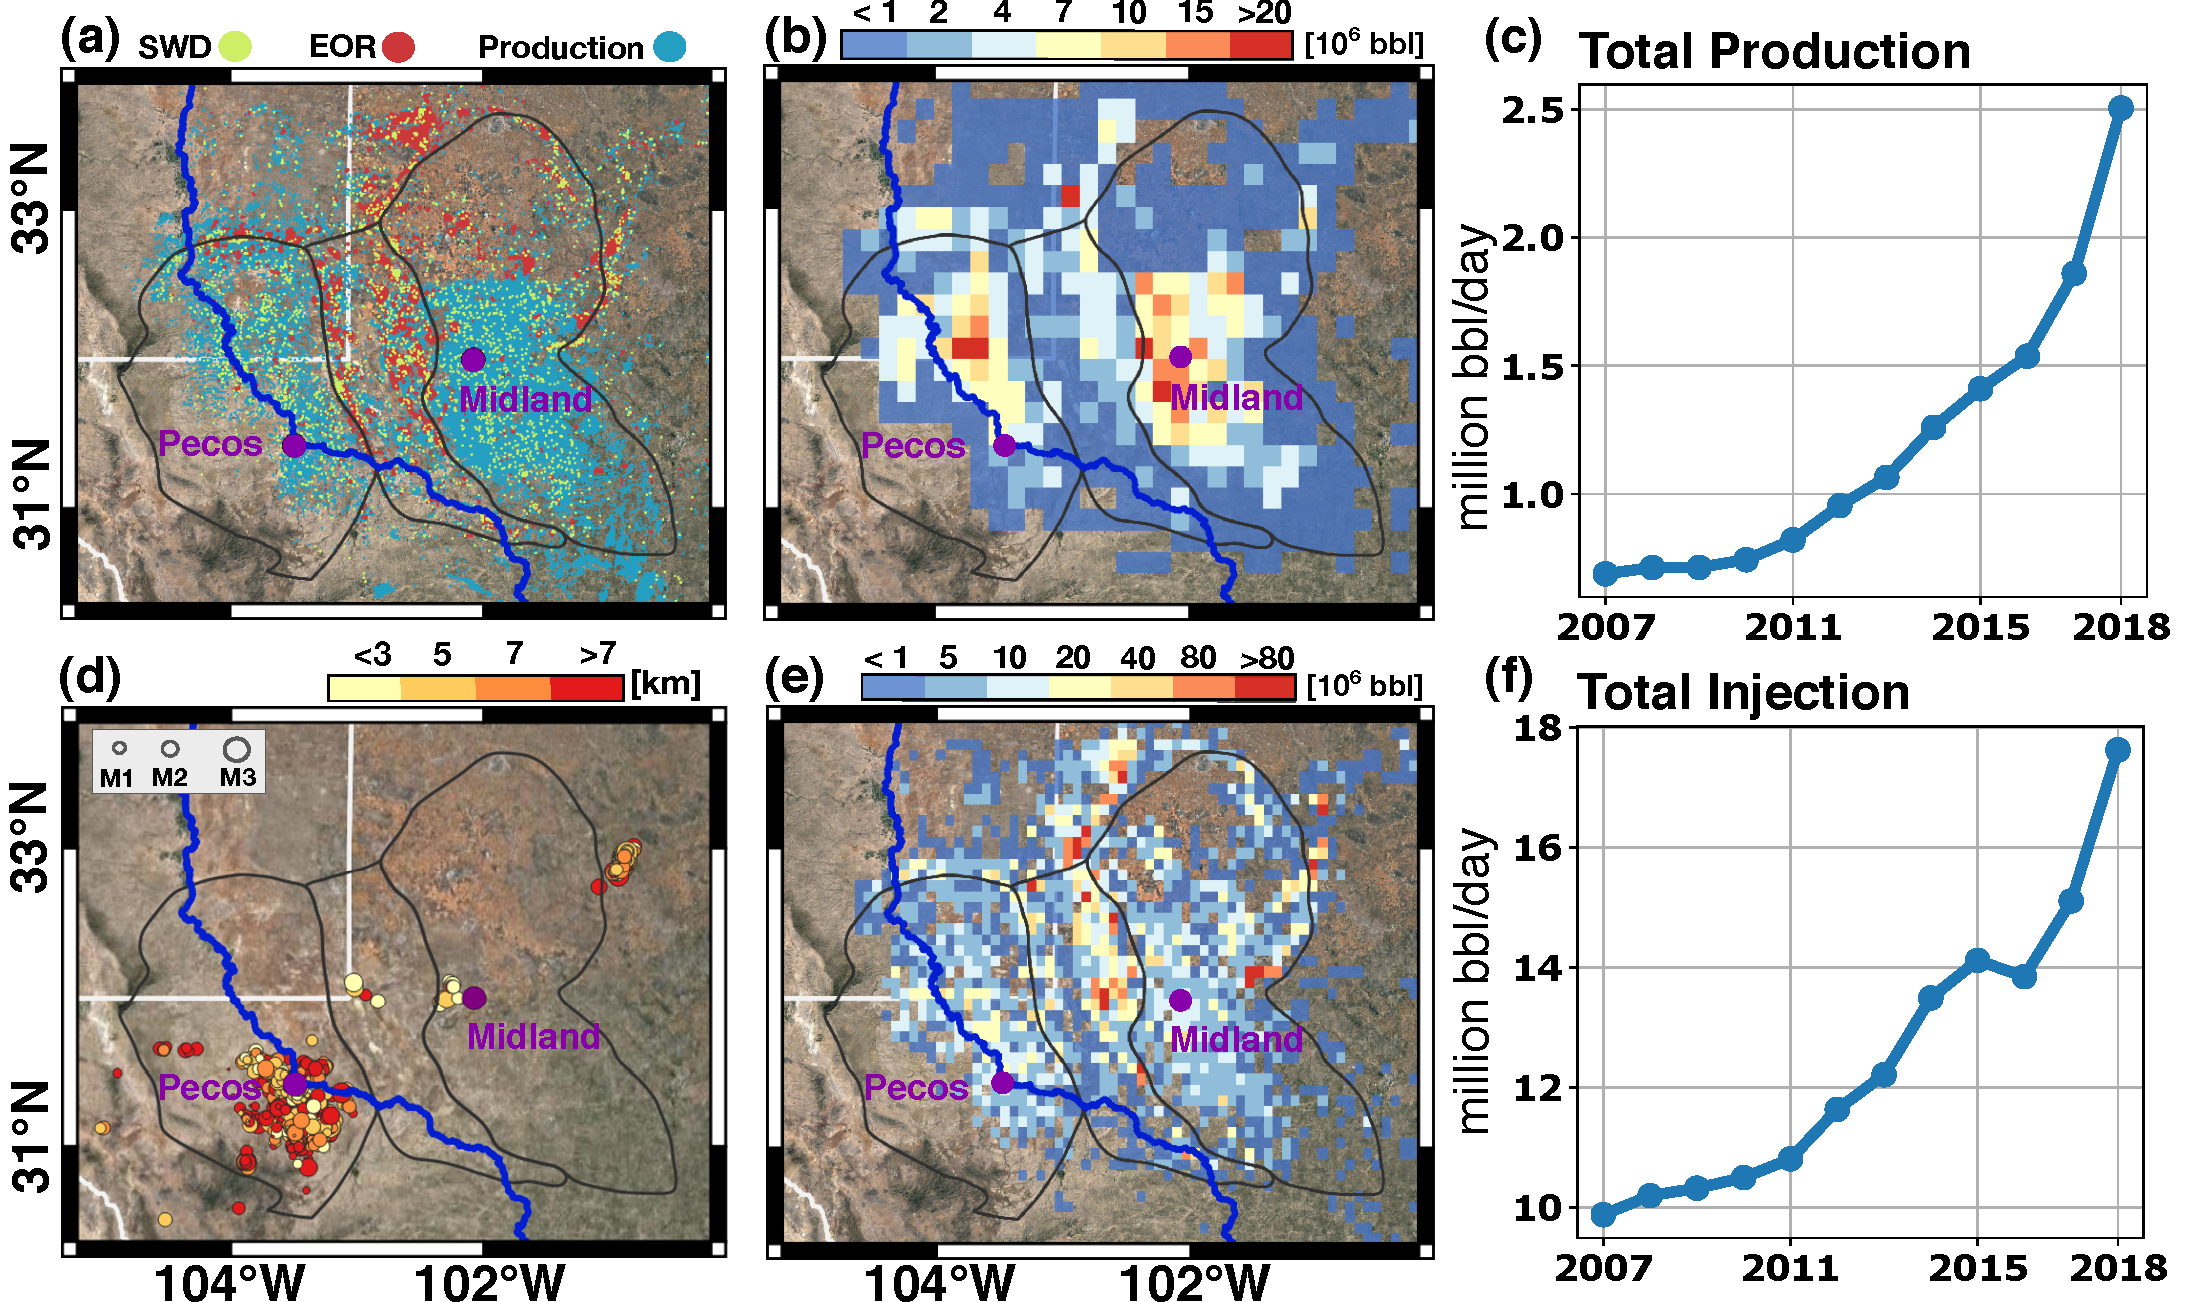
\includegraphics[width=0.99\linewidth]{figures/supplement/figureS1-cisr-data.pdf}
\caption{Shale development and induced seismicity in the Permian Basin. (a) Locations of oil production, enhanced oil recovery (EOR), and saltwater disposal (SWD) wells active in 2017. (b) Annual oil production volume on a 10-mile grid in 2017. (c) Permian region oil production rate as reported by the Texas Railroad Commission. (d) Locations of earthquake hypocenters detected by TexNet in 2017. The color and size of a circle indicates the estimated earthquake depth and magnitude. (e) Annual injection volume (including both SWD and EOR wells) on a 5-mile grid. (f) Permian region injection rate (including both SWD and EOR wells) as reported by the Texas Railroad Commission.
}
\label{fig:Permian}
\end{figure*}

\begin{figure}[!htbp]
\centering
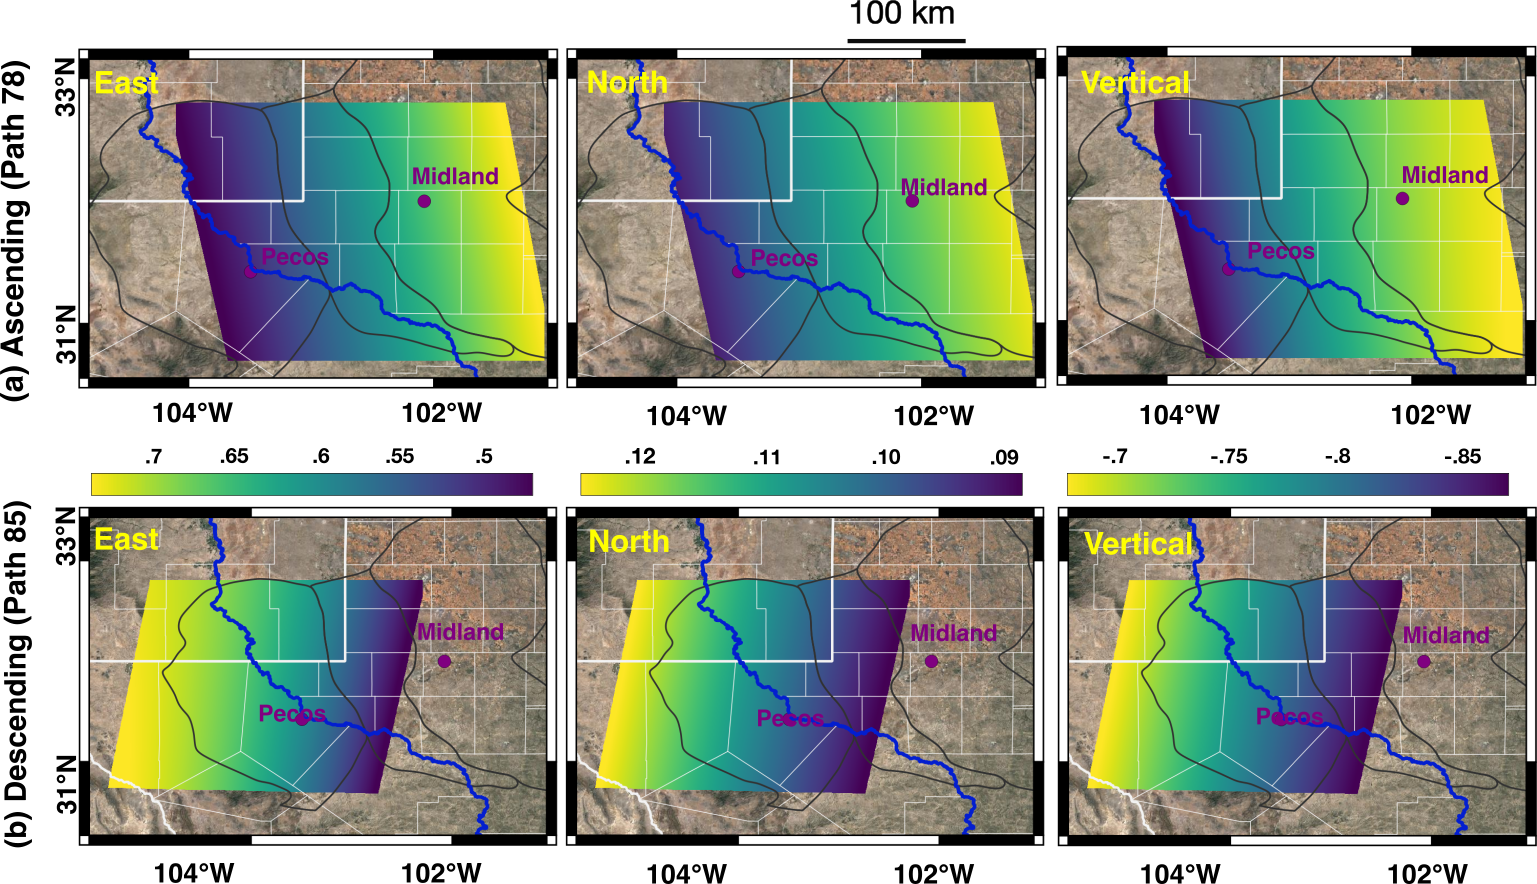
\includegraphics[width=.98\textwidth]{figures/supplement/figureS2-los.pdf}
\caption{East, north, and vertical coefficients of the line of sight (LOS) unit vector of all Sentinel-1 path 78 and path 85 pixels. Positive LOS direction points away from the satellite to the ground.}
\label{fig:los-map}
\end{figure}

\begin{figure}
\centering
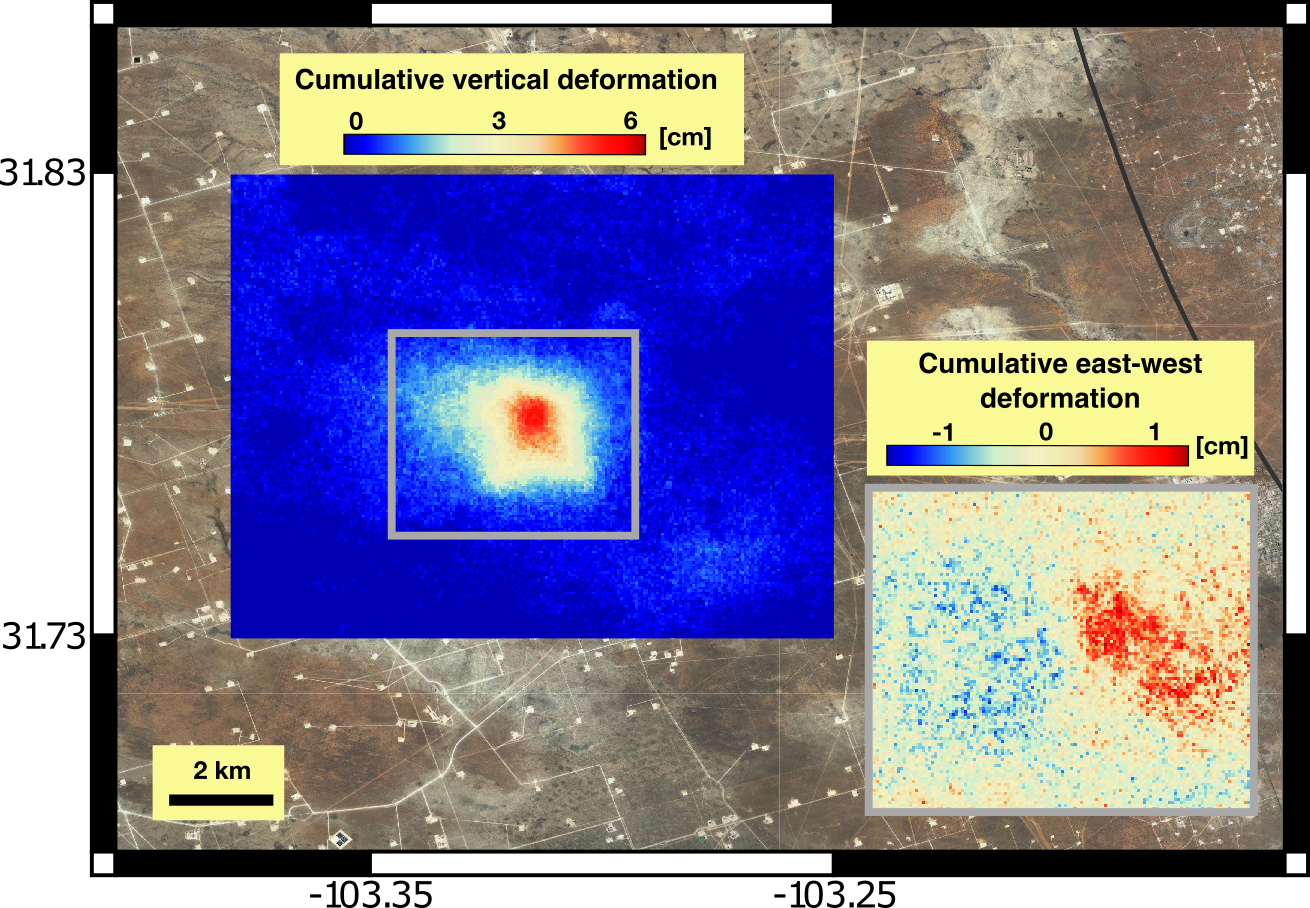
\includegraphics[width=\textwidth]{figures/supplement/figureS3-injection-kim-lu.pdf}
\caption{Cumulative surface deformation between November 2014 and April 2017 due to wastewater injection in Winkler County, TX. The horizontal motion here is $\sim$ 20\% of the vertical motion, with up to $\sim$ 5.5 cm of uplift and $\sim$ 1.2 cm of east-west motion. This localized deformation feature was originally reported in \citeA{Kim2018}.}
\label{fig:injection-kim-lu}
\end{figure}

\begin{figure}
\centering
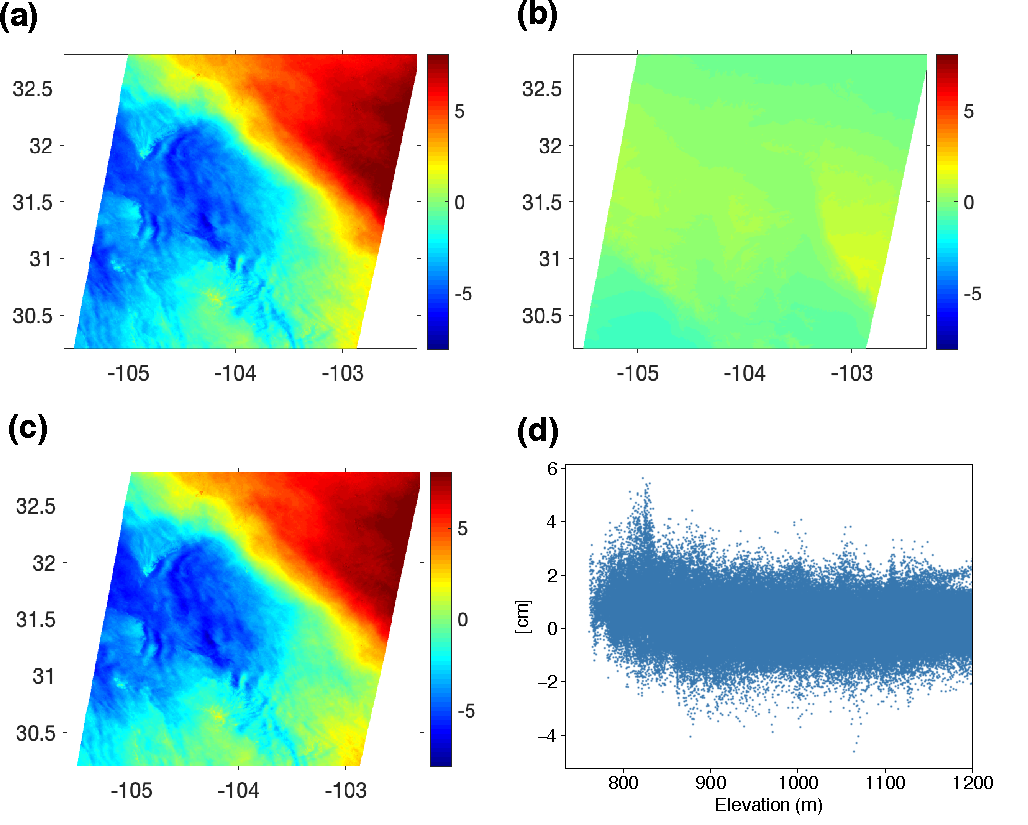
\includegraphics[width=\textwidth]{figures/supplement/figureS4-gacos.pdf}		
\caption{(a) LOS measurements (in cm) of a descending interferogram (20150127-20150220) before the GACOS correction. (b) GACOS tropospheric correction (in cm) for the 20150127-20150220 interferogram \cite{yu2018interferometric}. (c) LOS measurements (in cm) of a descending interferogram (20150127 - 20150220) after the GACOS correction. (d) LOS measurements (in cm) of the 20150127-20150220 interferogram vs. the Digital Elevation Model (DEM).}
\label{fig:GACOS}
\end{figure}

\begin{figure}
\centering
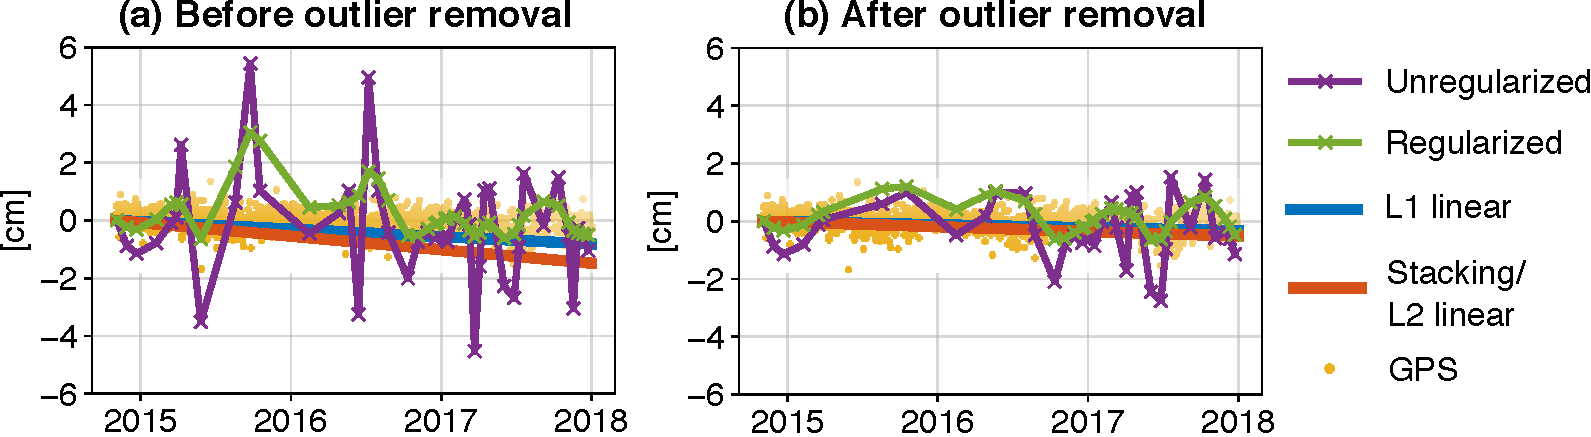
\includegraphics[width=\textwidth]{figures/supplement/figureS5-compare-insar-2panel.pdf}
\caption{Comparisons of InSAR unregularized SBAS time series (purple), regularized SBAS time series (green), linear deformation trend estimated by minimizing the $L_1$-norm of the residuals (blue), and the $L_2$-norm of the residuals/ stacking approach (red)  (a) before and (b) after removing LOS measurement outliers. ENU GPS data from station TXSO has been projected onto the radar LOS (orange dots).}
\label{fig:compare}
\end{figure}

\begin{figure}
\centering
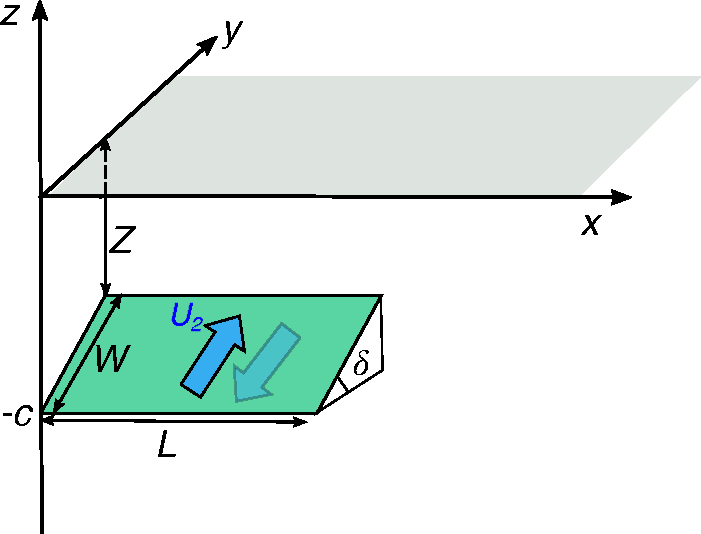
\includegraphics[width=\textwidth]{figures/supplement/figureS6-fault-geom.pdf}
\caption{A finite rectangular fault model \cite{Okada1992}. Here $U_2$ is the magnitude of dip slip (positive in reverse fault direction), $\delta$ is the dip angle, $Z$ is the depth to the top of the fault, $c$ is the depth to the bottom of the fault, $L$ is the length along the strike direction, and $W$ is the width along the dip direction.}
\label{fig:model-fault-geom}
\end{figure}

\begin{figure}
\centering
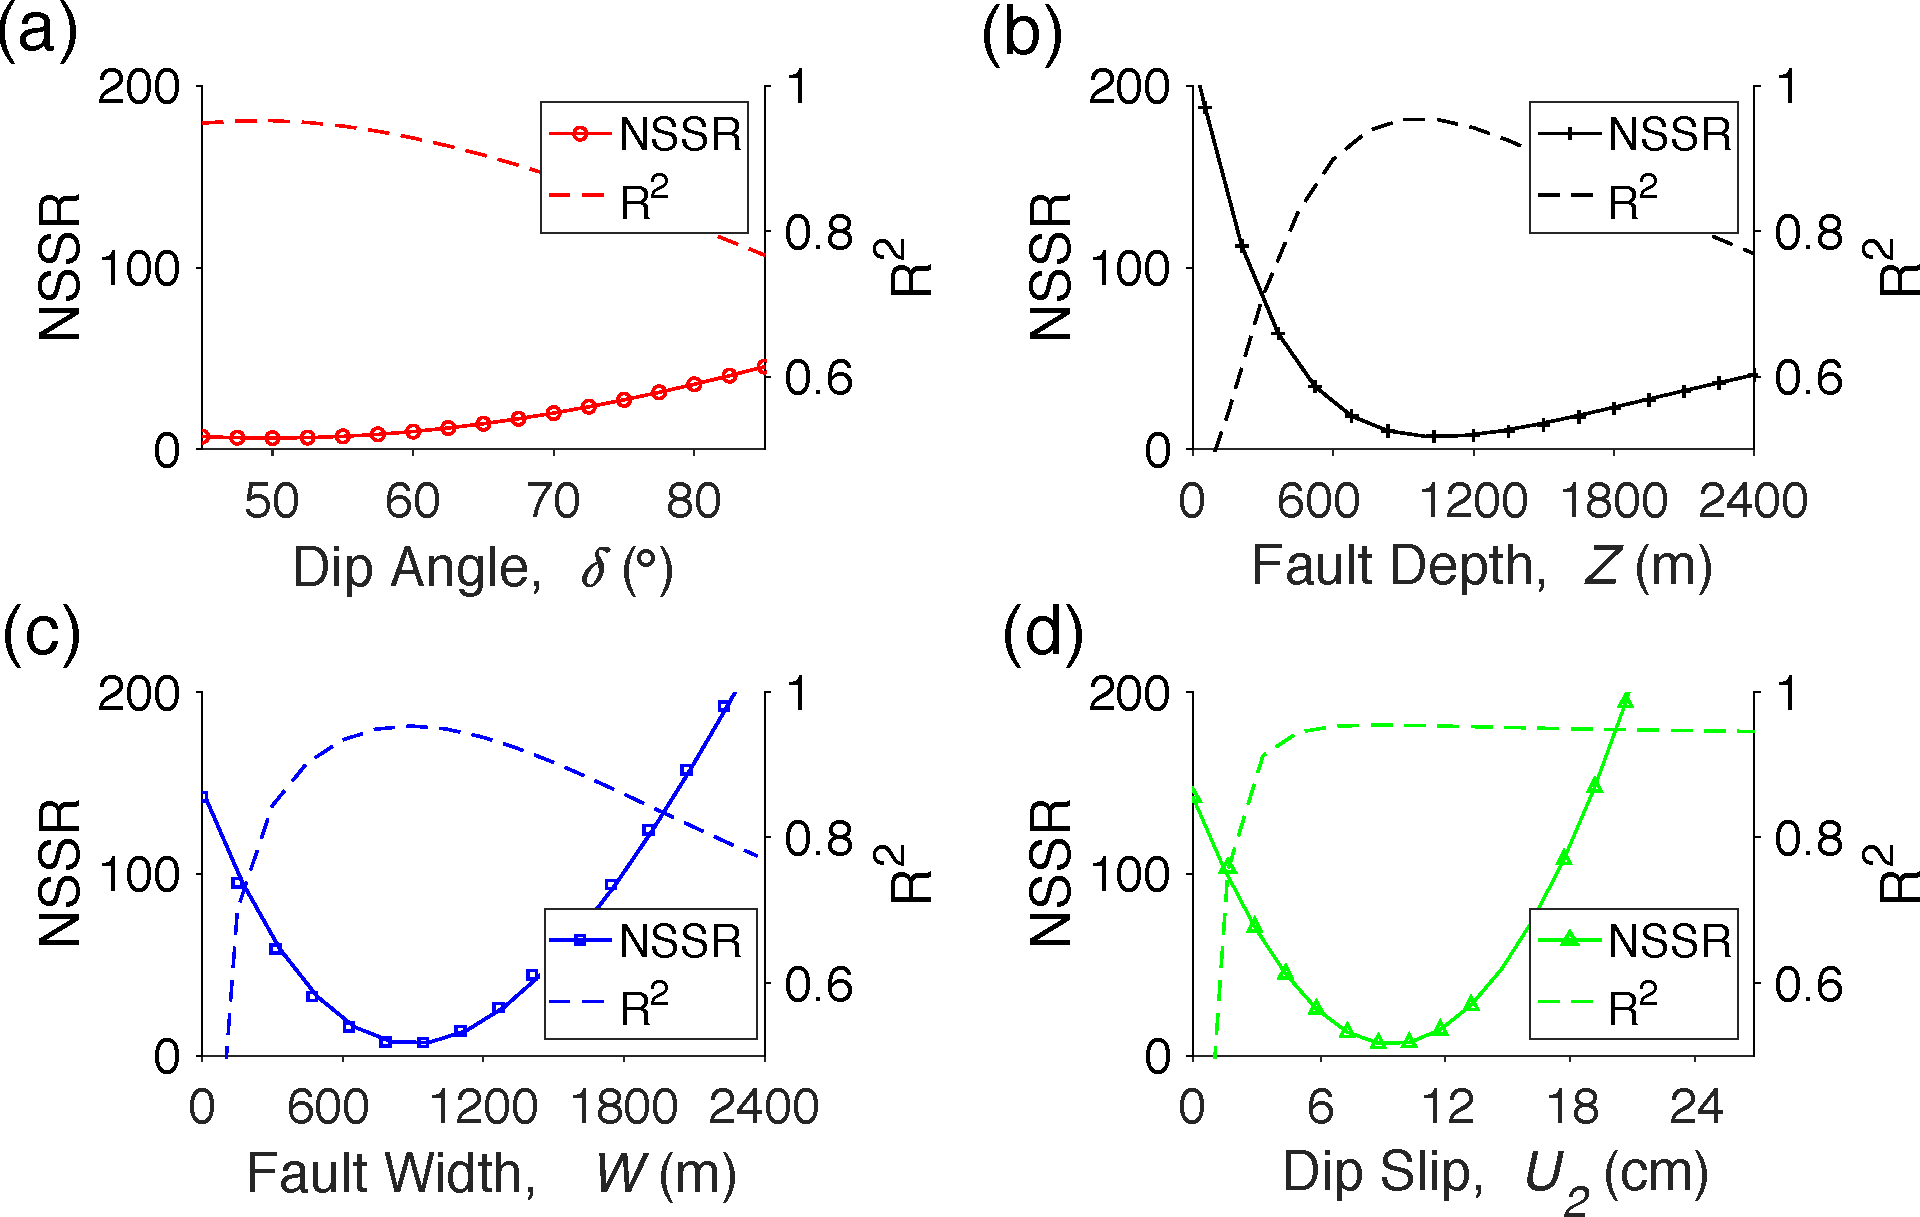
\includegraphics[width=.98\textwidth]{figures/supplement/figureS7-fault-supplement-nssr.pdf}
\caption{The Normalized Sum of Squared Residuals (NSSR) and R-squared ($ R^2 $) of fault \#3 relative to (a) fault dip angle ($ \delta $), (b) fault depth from the surface to the top of the fault ($ Z $), (c) fault width along the dip direction ($ W $), and (d) net dip slip magnitude ($ U_2 $).}
\label{fig:fault-supplement-nssr}
\end{figure}

\begin{figure}
	\centering
	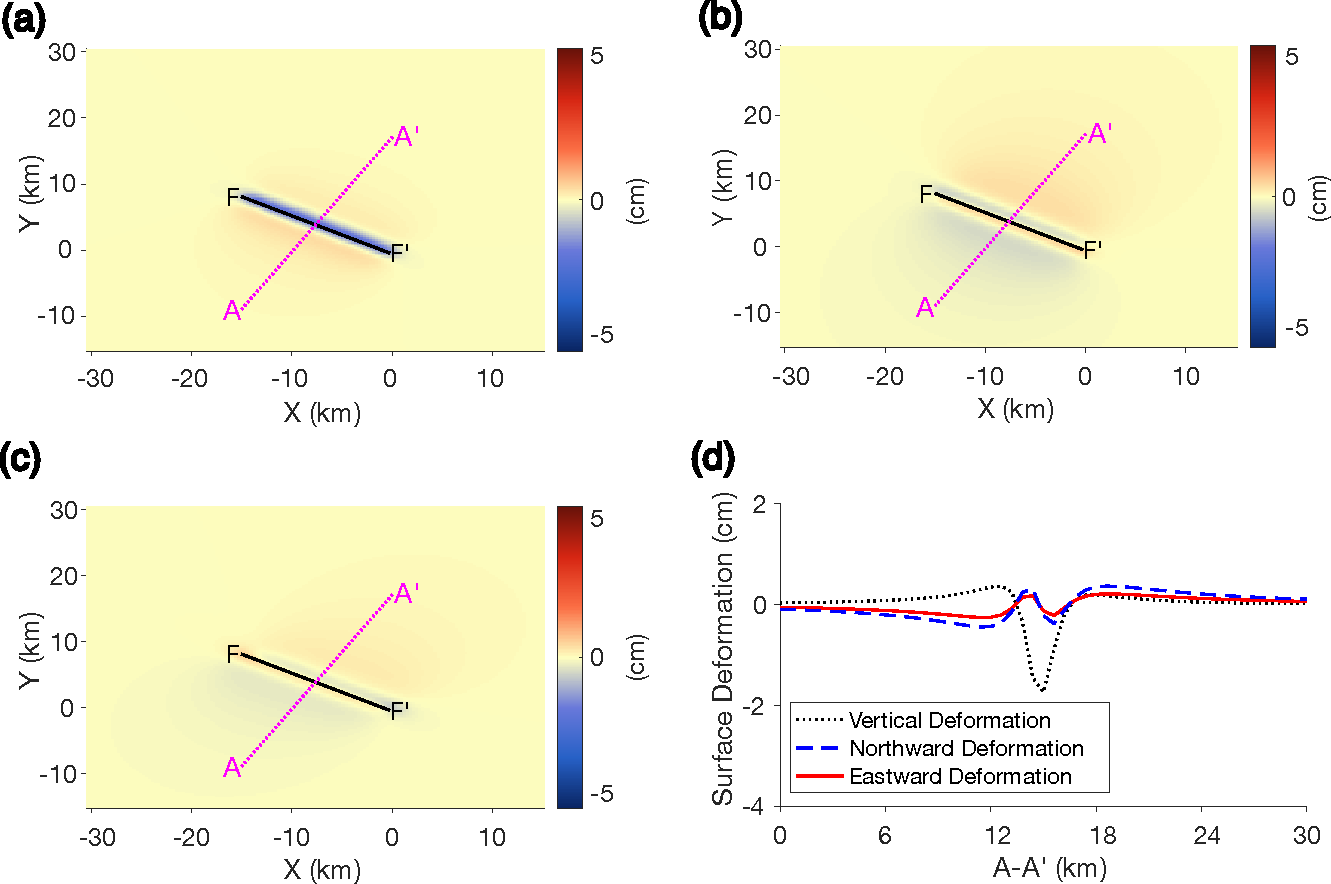
\includegraphics[width=\textwidth]{figures/supplement/figureS8-fault-predicted-xyz.pdf}
	\caption{The predicted surface deformation from the Okada fault model with best-fit parameters in the (a) vertical direction (positive means uplift), (b) northward direction (positive means north, negative means south), and (c) eastward direction (positive means east, negative means west). (d) Comparison of the 3D deformation profiles along A-A$^{'} $ transect that is perpendicular to fault plane.
	}
	\label{fig:fault-model-xyz}
\end{figure}

\begin{figure}
\centering
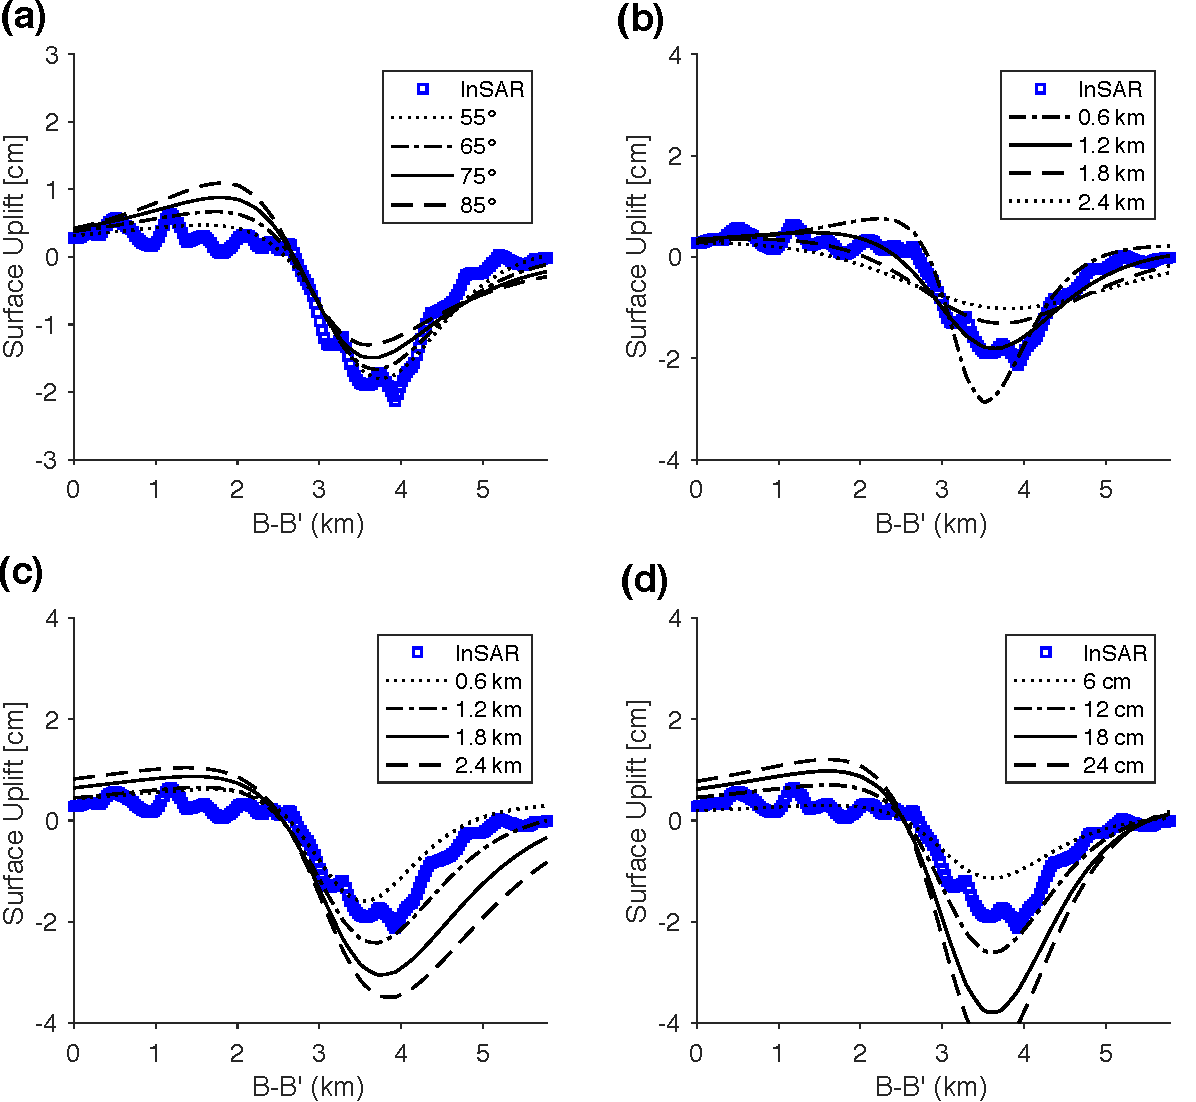
\includegraphics[width=\textwidth]{figures/supplement/figureS9-fault-supplement2.pdf}
\caption{Estimated surface subsidence along the B-B' transect associated with fault \#3 with various fault properties: (a) fault dip angle ($ \delta $) of 55$ ^{\circ} $, 65$ ^{\circ} $, 75$ ^{\circ} $, 85$ ^{\circ} $, (b) fault depth from the surface to the top of the fault ($ Z $) of 0.6 km, 1.2 km, 1.8 km, 2.4 km, (c) fault width along the dip direction, $ W $) of 0.6 km, 1.2 km, 1.8 km, 2.4 km, and (d) net dip slip magnitude ($ U_2 $) of 6 cm, 12 cm, 18 cm, 24 cm.}
\label{fig:fault-supplement2}
\end{figure}

\begin{figure}
	\centering
	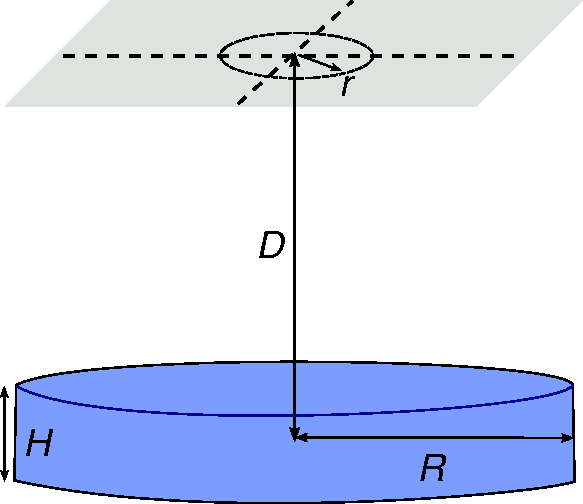
\includegraphics[width=.8\textwidth]{figures/supplement/figureS10-reservoir-geom.pdf}
	\caption{
	Geometry of reservoir model in \citeA{Geertsma1973}, where $H$ is the reservoir height, $D$ is the reservoir depth, and $R$ is the reservoir radius.
	}
	\label{fig:model-reservoir-geom}
\end{figure}

\begin{figure}
	\centering
	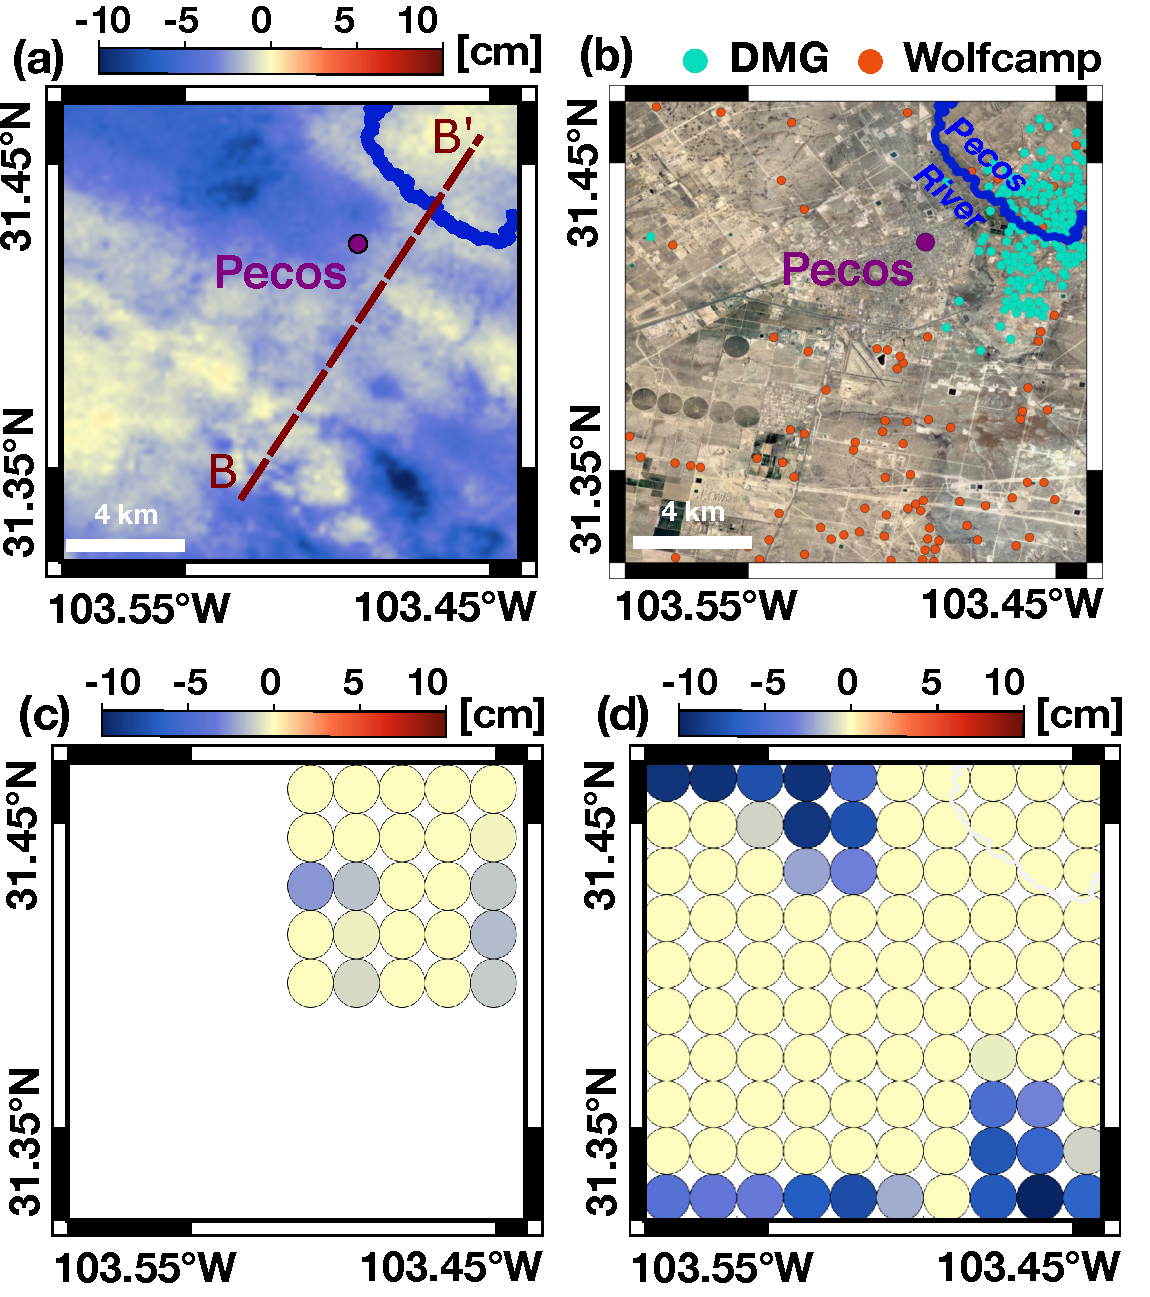
\includegraphics[width=\textwidth]{figures/supplement/figureS11-reservoir-wells.pdf}
	\caption{(a) Input for reservoir model: vertical surface deformation difference between InSAR and fault model (vertical surface deformation not explained by the fault model). (b) Producing well locations in near Pecos in the Delaware Mountain Group (DMG, cyan) and Wolfcamp (orange). Reservoir compaction values in (c) DMG reservoirs at depth 1.52km, and (d) Wolfcamp reservoirs at depth 3.05km. 

	}
	\label{fig:model-reservoir-wells}
\end{figure}


\begin{figure}
	\centering
	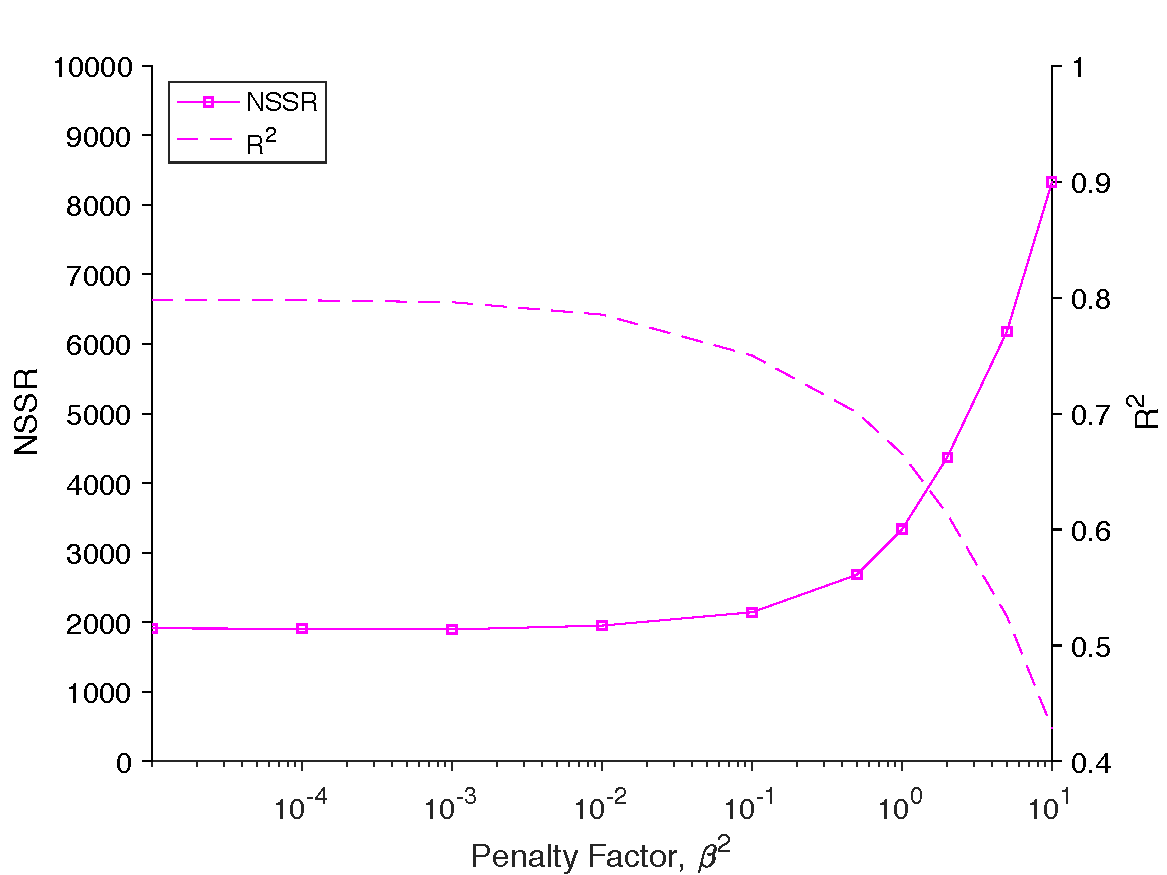
\includegraphics[width=\textwidth]{figures/supplement/figureS12-reservoir-nssr.pdf}
	\caption{The Normalized Sum of Squared Residuals (NSSR) and R-squared ($ R^2 $) with varying penalty factor ($ \beta^2 $) for the discretized reservoir compaction model
	}
	\label{fig:model-reservoir-nssr}
\end{figure}

%\bibliography{permian,insar} 
\bibliography{StaniewiczGRL} 

%% ------------------------------------------------------------------------ %%
%
%  END ARTICLE
%
%% ------------------------------------------------------------------------ %%
\end{article}
\clearpage

\end{document}


